\section{四种广角偏移方法}
本节所述反射地震资料的四种偏移方法均为现代生产环境中出现的方法。它们是易于处
理广角射线问题的一类方法,同时又是难以应用于处理速度横向变化问题的一类方法。

\subsection{旅行时间深度}
偏移处理程序的输出,理想的应是$(x,t)$平面中的图像,可实际上垂直坐标轴几乎从
来不是深度$z$,而是垂直旅行时间$\tau$。在恒速地层情形下,该时间与该深度由一
个比例因子联系起来,比例因子的意义就是:与$(x,t)$平面相比$(x,\tau)$平面的垂
直比例放大了。在地震普查工作中,垂直方向往往放大五倍左右。到了业已充分缩小
勘探范围以便定井位的时候,采用的垂向放大比例因子很可能是1左右(即没有放大)。

旅行时间深度$\tau$的定义通常包括波下行传播和上行传播二者的时间,这相当于使岩
层速度隐含有因子2。地震时间剖面一般是按爆炸反射面波场解释的,为使之一致,在
波场分析时要使岩层速度$v_{true}$减半,即
  \begin{equation}
  \tau=\frac{2z}{v_{true}}=\frac{z}{v_{half}}
  \label{eq:ex1.3.1}
  \end{equation}
地震资料解释中的第一项任务就是计算出垂向放大的近似数值。这个数值恐怕不会打印
在数据说明中,因为速度还未真正已知。再者,速度通常随深度而增大,意昧着垂向放
大随深度而减小。对于速度分层介质,时深转换公式为 
\begin{gather}
\tau(z)=\int_{0}^x\frac{dz}{v(z)} \notag \\ 
\frac{d\tau}{dz}=\frac{1}{v} \label{eq:ex1.3.2}
\end{gather}

\subsection{绕射扫描与等时线扫描}


绕射扫描与等时线扫描\footnote{原文中的hyperbola-summation method
按国内现已熟悉通用的术语,译为绕射扫描,semicircle-super-position method
则译为等时线扫描。——译者}是所有已知方法中最易于理解的偏移方法。

$(x,z)$空间内的圆或$(x,t)$空间内的双曲线这类圆锥截面的方程为
\begin{subequations}
\begin{equation}
z^2+x^2=v^2t^2
\label{eq:ex1.3.3a}
\end{equation}

转换为旅行时间深度$\tau$时,则

\begin{equation}
\tau^2+\frac{x^2}{v^2}=t^2
\label{eq:ex1.3.3b}
\end{equation}
\end{subequations}
式中,$v$为速度。
图\ref{fig:omk/schneider}是等时线扫描方法的图解说明(图件及其标题说明均取自
Schneider的经典论文〔1971〕)。取数据场使之包含有少量几个脉冲函数时,输出应
是适当的一些半圆之叠加结果,各个半圆代表单个脉冲所形成的那种球形反射面地层模
型。取数据场为各具有一千个采样点的一千个地震记录道时,则输出就是一百万个半圆
的一种叠加结果。既然地震记录既有正极性又有负极性,于是半圆将半数是以负极性叠
加,最终叠加结果看起来差不多会很像个样子。确实,除了在$(x,\tau)$空间内的一个
孤立脉冲之外,各半圆几乎处处都可能彼此相互抵销。发生这事,你可能会正确地猜出:
$(x,t)$空间内的输入数据剖面就是一种惠更斯二次震源,即能量是沿一双曲线集中分布
的。这点将引导我们转向绕射扫描方法的讨论。

偏移的绕射扫描方法如图所示。方法的基本思想是要在$(x,\tau)$空间的某个时间上用
扫描办法形成一个点,而不是像等时线扫描方法那样,把一百万十半圆彼此叠加在一起
逐点形成$(x,\tau)$空间内的各个点。为在$(x,\tau)$空间的输出结果中形成一个固定
点,试想像有式\ref{eq:ex1.3.3b}所示的一种双曲线,使其顶部位于$(x,\tau)$空间的
相应位置上。把该双曲曲所接触到全部数据值相加起来,所产生的值就作为$(x,\tau)$
空间内适当位置上的输出结果。按同样方法将$(x,\tau)$空间内所有其他位置均填满。

\begin{figure}[H]
\centering
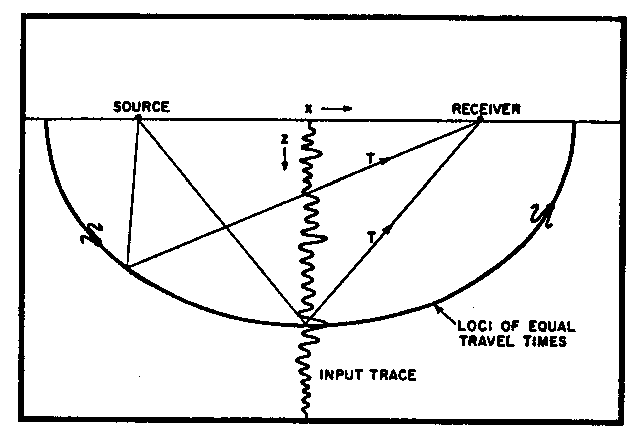
\includegraphics[width=0.5\textwidth]{omk/schneider}
\caption[schneider]{等时线扫描方法示意图。图中所示代表按炮检距中点位置的深度
(也可用时间)显示的一个输入记录道所发生的过程。将这个记录道各个振幅值沿一个曲
线分布,构制成地下界面,该曲线代表震源至反射点再至接收器的旅行时间为常数之各
点的轨迹。如速度为常数,则这些曲线是以踩源与接收点为焦点之椭圆。按这神处理办
法构成的图形,简单说就是以记录道振幅信息调制的波阵面图。它本身显然不是一个有
用的界面映像,但是当由相邻一些记录道(不同炮检距的共深度记录道)的类似图形构
制成图时,由于在古典的惠更斯原理意义上的波阵面之间发生相长干涉与相消干涉。就
产生了有意义的地下界面映像。例如,相邻记录道的波阵面会全部相交于一个绕射源上,
相长叠加而形成以强振幅斑点形式出现的一个绕射体映像,其垂向与水平方向的分辨率
由脉冲频宽及水平扫描半径所控制。另一方面,在有反射界面情形下。来自邻近记杂道
的波阵面均与该界面相切,从面由于相邻波阵面重叠部分的相长干涉而形成反射面映像。
在没有反射体与散射体之界面的区域内,波阵面由于随机叠加而趋于抵销}
\label{fig:omk/schneider}
\end{figure}
\begin{figure}[H]
\centering
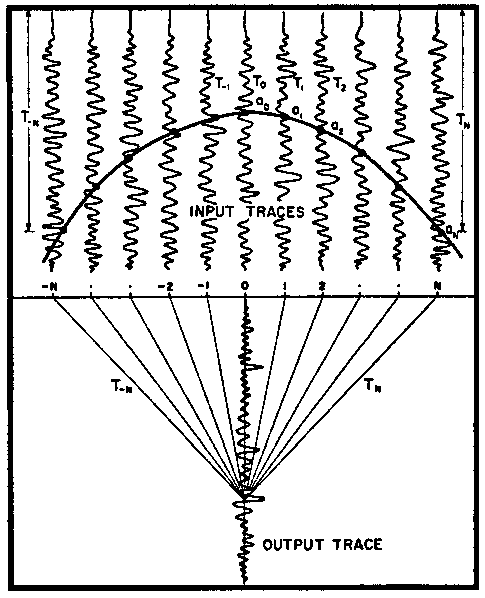
\includegraphics[width=0.5\textwidth]{omk/schneider2}
\caption[schneider2]{绕射扫描方法示意图。这个处理过程代表如何由图上部所示多次
叠加记录道组成的输入记录道集合产生出一个输出道记录道,图下部的输出记录道是反映
如何沿所示旅行时间曲线进行振幅求和而得出$(x,z)$点上的各个振幅值。这个曲线定义
为绕射双曲线。如果在所示输出点上的地下届面中存在有一个绕射源,则在该点将应形成
强振幅。这个过程也适用于反射面,因为一个反射面可以看成是连续的一系列绕射源,其
各自的映像合并产生一光滑连续分界面}
\label{fig:omk/schneider2}
\end{figure}

我们可以怀疑绕射扫描方法究竟是比等时线扫描方法好一点还是坏一点,或者它们是否
是等价的,相反的数据处理过程------或根据数据来建立模型——就是根据模型构制合成
记录。把以上所述两种偏移处理程序作一点改变,就可以变成模拟程序,这时,你不是
进行双曲线求和(译注:即绕射扫描hyperbola summation)或半圆叠加(译注:即等时
线扫描semicircle superposition),而是进行双曲线叠加(hyperbola superposition)
或半圆求和(semicircle summation)。我们也可以怀疑上述两种偏移处理程序是否真正
就是模拟程序的逆过程。有一些需要加以考虑的因素:
\begin{itemize}
\item 惠更斯二次震源波形振幅对角度的依从关系(即倾斜函数);
\item 能量所受球面发散影响;
\item 惠更斯二次震源波形所受相移影响。事实证明,即使将这些复杂因素忽略不计,
  所得处理结果还是相当好的。
\end{itemize}


随着其他一些偏移方法的发展,这些早期偏移方法的缺陷被了解得更为深入,并且发现
只要仔细处理,大部分缺陷是可以改正的。后期发展的一些偏移方法有一个好处,那就
是它们实现了真正的全通滤波(all-pass filter)。这样一类偏移方法保存了资料数据的
一般外貌,这点可以认为是由于恢复了沿双曲线积分所破坏了的高频成分。Trorey(
1970)与Hilterman(1970)利用Kirchhoff绕射积进行的工作导致了正演模拟程序,这项工作
成果终于提出了使绕射扫描方法与其他偏移方法能够符合一致(至少对于恒速情形是如此)
的定量手段(Schneider, 1977)。现今的用术语中将任何绕射扫描或等时线扫描方法都称作
Kirchhoff法,而严格地讲,Kirchhoff分仅能应用于恒定速度的情形。

\subsection{空间假频现象}
空间假频现象意味着沿空间坐标轴的数据采样不足,这种困难如此普遍存在,所有偏移
方法都必须考虑它的影响。

数据应按每波长多于两个点进行采样;否则波至方向就变得难以捉摸。图\ref{fig:omk/alias}
所示是沿$x$轴采样密度不足的合成数据,你可看出,在高频和陡倾角时,假频问题变得
很严重了。
\begin{figure}[H]
\centering
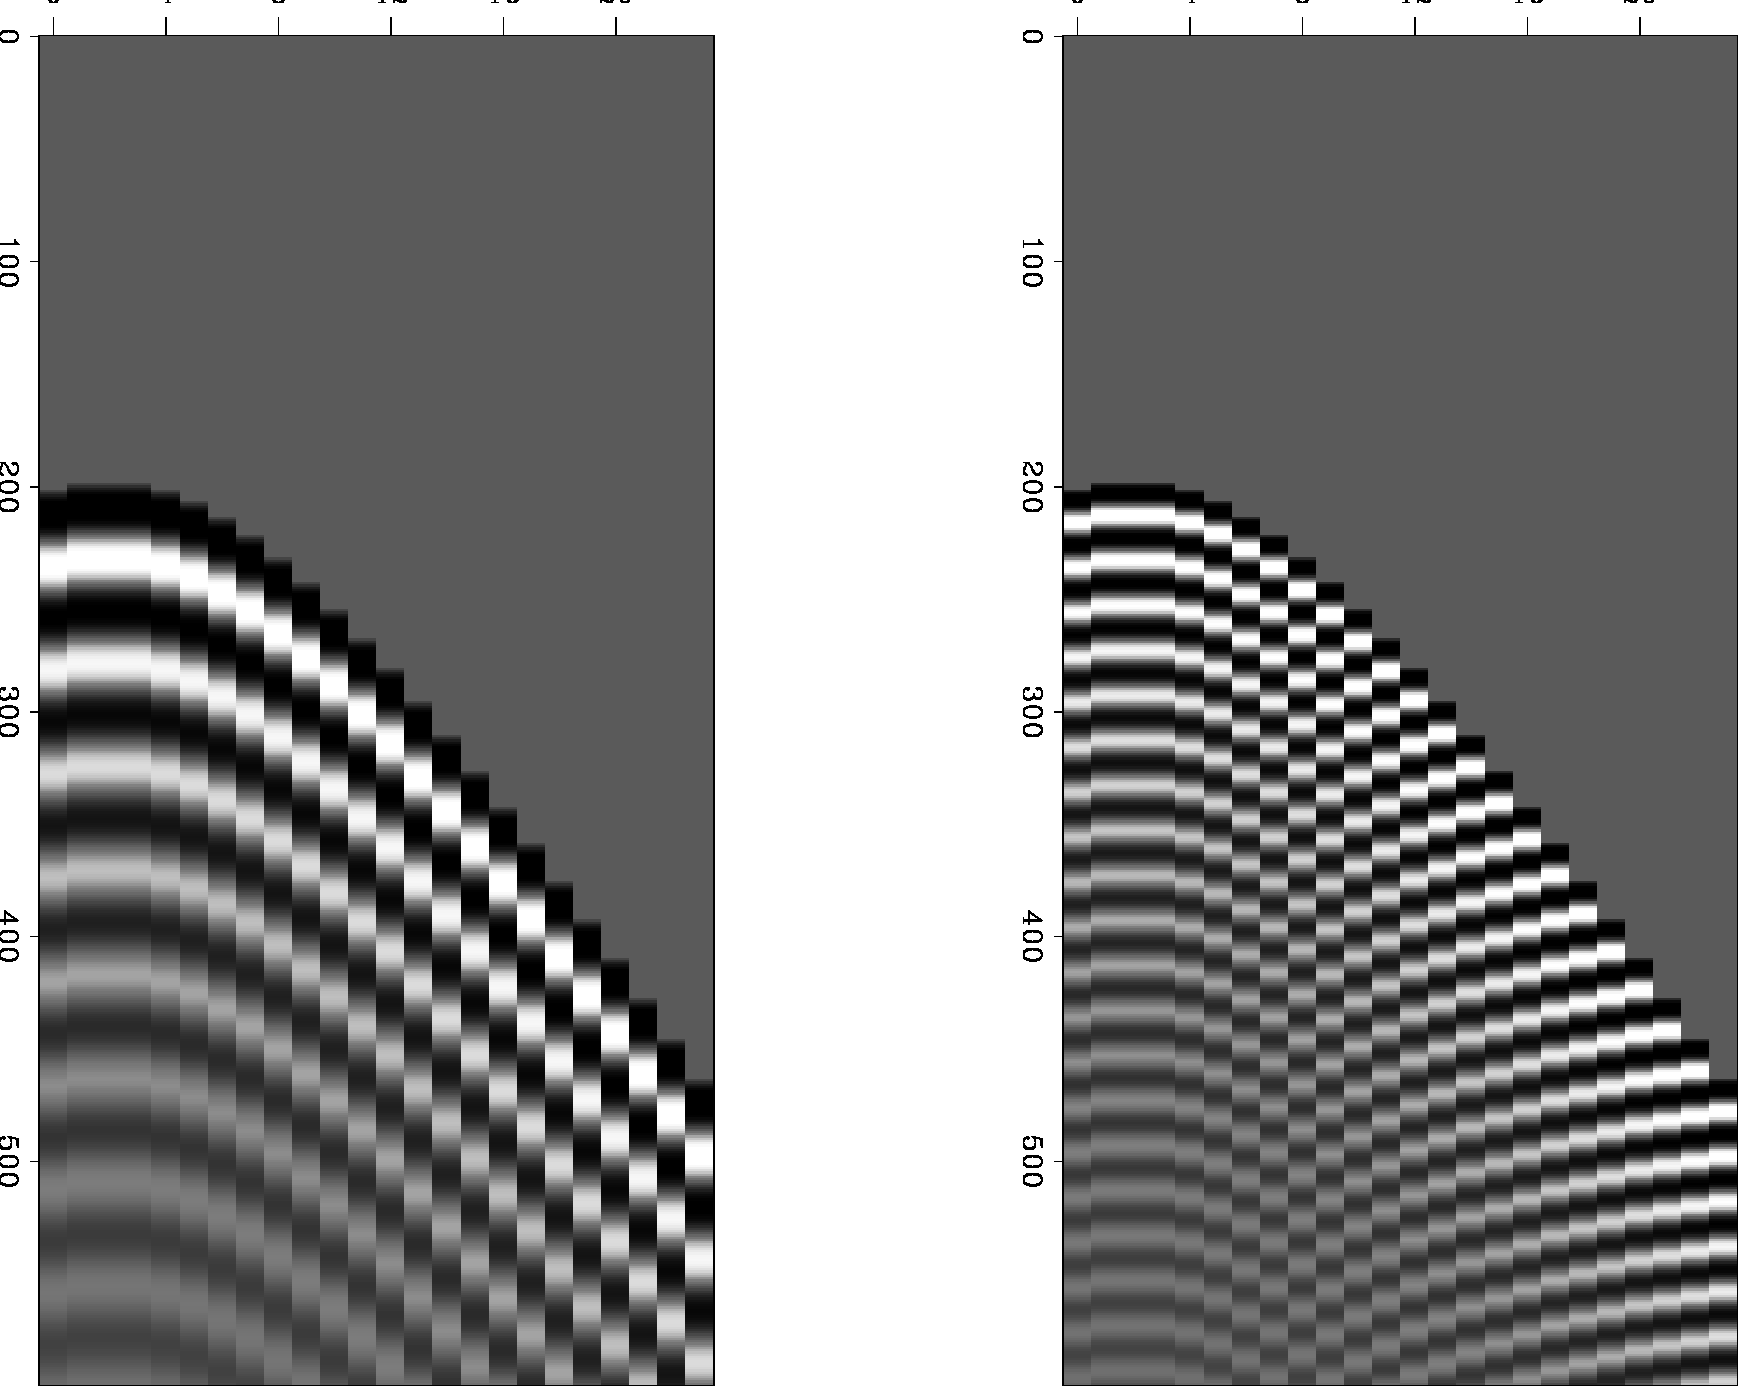
\includegraphics[width=0.95\textwidth]{omk/alias}
\caption[alias]{空间采样不足的合成数据。为更好地看出初至角度的模糊程度,
可从图侧以掠射角度来看}
\label{fig:omk/alias}
\end{figure}
对受空间假频影响的资料进行偏移,现在还没有什么普遍适用的可以自动校正其影响的
方法,在这类场合下,人可能比机器做得更好,因为人在识别真斜率时是很熟练的。然
而,当资料经过适当采样处理时,以波动方程为基飿的计算机偏移方法得出的结果还是
比人工方法强多了。当代地震勘探通常都是沿测线进行适当采样的,不过在垂直方向往
往存在困难。

各种绕射扫描型的偏算手苯5曼空间假频影响的危险,应该仔细处理以求避免这点。首
先要认识到,你应该沿双曲线的轨迹进行积分。每记录道只有一个采样点参与的求和过
程,是一种很粗略的近似,最好像图\ref{fig:omk/lineint}所示那样使更多采样点参
与求和。在双曲线呈陡倾斜之处,算子受假频影响的可能性就增大。在生产中,受假频
影响的算子往往是出现在海底反射之上,尽管海底可能是平坦的,可是由于双曲线的陡
倾斜翼穿过海底反射,于是算子在那里就获得了一种受干扰的外貌特征。
\begin{figure}[H]
\centering
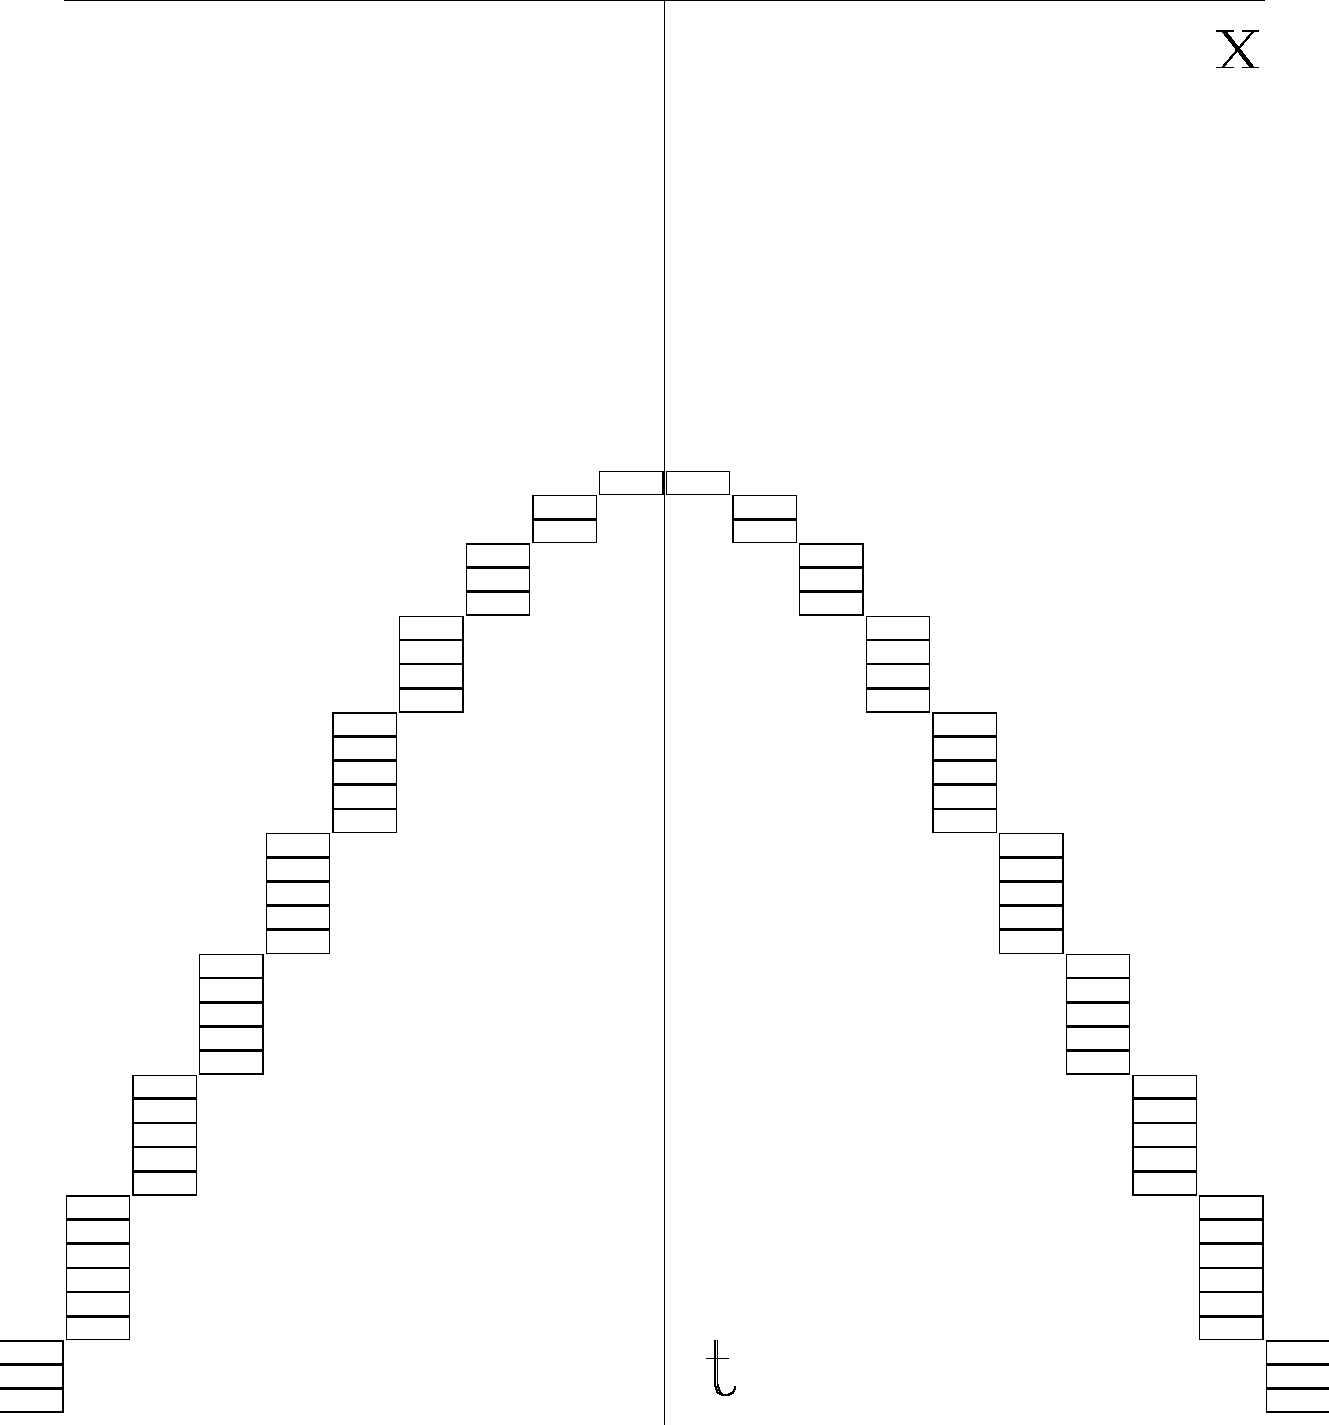
\includegraphics[width=0.6\textwidth]{omk/lineint}
\caption[lineint]{对于低速双曲线轨迹,积分将需要记录道多于一个采样点}
\label{fig:omk/lineint}
\end{figure}

\subsection{相移偏移方法(Gazdag法)}
相移法用$\exp(ik_xz)$直接进行向下外推,然后估算$t=0$时(反射面在$t=0$时激发)的
波场。所有广角偏移方法中,属它最容易处理速度随深度变化的问题了,即使是相位角
和倾斜函数的影响,也都能正确地自动包括在内。同$Kirchhoff$偏移方法不一样,采用
这种相移法不存在使算子出现假频的危险。

相移法开始是对时间剖面进行二维傅氏变换(关于二维傅氏变换的某些实际细节,在1.7
节内讨论),然后把所有在$(\omega,k_x)$平面内的变换后的数据值乘以下式
\begin{equation}
e^{ik_z\Delta z}=exp\{-i\frac{\omega}{v}[1-(\frac{vk_x}{\omega})^2]^{1/2}\Delta z\}
\label{eq:ex1.3.4}
\end{equation}
向下延拓至某一个深度$\Delta z$。输出偏移剖面的时间采样间隔$\Delta\tau$通常选
择为等于输入数据的时间采样率(往往是4毫秒),所以,选取深度为$\Delta z=v\Delta\tau$
时,一个时间单位情形下的向下延拓算子为C,数据将多次乘以C,从而就是将它向下延拓
了许多$\Delta\tau$步长。
\begin{equation}
exp\{-i\omega\Delta\tau[1-(\frac{vk_x}{\omega})^2]^{1/2}\}=C
\label{eq:ex1.3.5}
\end{equation}
其次的任务是成像.在每个深度上完成一个逆傅氏变换之后,接着就选定其在$t=0$时的
值(反射面在$t=0$时激发)。很幸运,仅需在$t=0$时的一个点上完成傅氏变换,所以
这也就全部所需要的计算了。由于$t=0$时的值只是各个$\omega$频率分量之和,计算
特别容易(将$t=0$代入逆傅氏积分就可知道)。最后就是进行$k_x$至$x$的逆傅氏变
换。从上行波$u$计算出映像的偏移过程可以总结如下\footnote{关于RATFOR程序的说
明,见1.7节。括号符号${\ldots\ldots}$内为语句,符号$FT[\ldots\ldots]$表示对
符号$[\ldots\ldots]$内的函数完成傅氏变换。——译者}:\\
$U(\omega,k_x)$=FT[u(t,x)]\\
For $\tau=\Delta\tau,2\Delta\tau,\ldots\ldots$, end of time axis on seismogram\{\\
For all $k_x$ \{\\
 Image$(k_x,\tau)$ = 0.\\
		For all $\omega$ \{\\
			C = $exp(-i\omega\Delta\tau\sqrt{1-v^2k_x^2/\omega^2})$\\
			U$(\omega,k_x)$ = U$(\omega,k_x)$*C\\
			Image$(k_x,\tau)$=Image$(k_x,\tau)$+U$(\omega,k_x)$\\
		\}\\
	\}\\
	image$(x,\tau)$ = FT\{Image$(k_x,\tau)$\}\\
\}\\
逆偏移(即正演模拟)的处理与此非常箱似,从很大深度上其值为零的上行波开始,乘
以$exp(ik_x\Delta z)$,按步长将该波向上推进;随着通过地层的每个深度水平,由各
该深度水平上形成的爆炸反射面就不断加进上行波内。模拟上行波$u$的程序为:\\
$Image(k_x,z)$=FT[image(x,z)]\\
For all $\omega$ and all $k_x$\\
	U$(\omega,k_x)$=0.\\
For all $\omega$ \{\\
For all $k_x$\{\\
For z=$z_{max}, z_{max}-\Delta z, z_{max}-2\Delta z, \ldots\ldots, 0$\{\\
	C = $exp(+i\omega\Delta z\sqrt{v^{-2}-k_x^2/\omega^2})$\\
	U$(\omega,k_z)$ = U$(\omega,k_z)$*C+Image$(k_x,z)$\\
	\}\}\}\\
u(t,x) = FT\{U$(\omega,k_x)$\} \\
复指数内取正号是由于对上行波和向上外推需各取一次负号的综合结果;关于$\omega$
、$k_x$和$z$的三种循环是可互换的,当速度$v$是深度的一个恒定函数时,把复指数
$C$的计算移到关于$z$的内循环之外去进行,可以加快程序的运行。

速度很难总是精确已知,所以,尽管它可能是随深度而稳定増大的,但往往还是在一些
层内按常数来近似处理,而不是按地震记录上每一千个左右的时间点作缓慢改变。这种
近似处理的好处是节省计算的时间。式\ref{eq:ex1.3.5}内的平方根和正弦与余弦一旦
已计算出,就可以多次重复利用式$\ref{eq:ex1.3.5}$所示复数乘因子,采用4毫秒的
采样率和200毫秒的层厚,该复数乘因子能一直使用50次而后才放弃。

\subsection{Stolt方法}
在大多数计算机上,Stolt偏移方法是有充裕余地的一种最快速的方法。就它的许多应
用而言,这点将是它最重要的特征。对于恒速地层情形,它是严格而又正确地同惠更
斯二次波源概念一致。像其他方法一样,这种偏移方法也可以使之颠倒而成为正演模
拟程序。有一个涉及原理问题的缺点,就是Stolt方法处理不了涉及速度随深度而变动
的问题。采用坐标轴拉伸处理(见4. 5节)来进行近似校正时种缺点就;能很大部分在
到补偿。还有一个实际应用上的问题,即所有傅氏变换都具有周期性。从原理上说,
这完全不成问题,因为在数据周围适当充填以零值就可以解决它。

Stolt方法可简单表示如下:\\
$p(x,t)\rightarrow P(k_x,\omega)\rightarrow(k_x,k_z=\sqrt{\omega^2/v^2-k_x^2})\rightarrow(x,z)$\\
现在看一看为什么要这样作.根据波场向下延拓的输入输出关系
\begin{equation}
P(\omega,k_x,z)=e^{ik_zz}P(\omega,k_x,z=0)
\label{eq:ex1.3.6}
\end{equation}
完成二维逆傅氏变换,得 \\
$P(t,x,z)=\iint e^{ik_xx-i\omega t+ik_zz}P(\omega,k_x,0)d\omega dk_x$\\
应用$(x,z)$点上的映像就是时间$t=0$时的爆炸反射面的这种思想,即得
\begin{equation}
Image(x,z)=\iint e^{ik_xx}e^{ik_z(\omega,k_x)z}P(\omega,k_x,0)d\omega dk_x
\label{eq:ex1.3.7}
\end{equation}
上式给出了最终的映像,但是它却是以一种不受欢迎的形式出现的。因为它暗示着必须
对每个深度$z$水平来完成一项二维积分。Stolt处理过程就是将如式\ref{eq:ex1.3.7}
所暗示的三维计算转换成一个二维傅氏变换。

到现在为止,还完全没有详细说明如何用上行波来代替下行波。波的方向是根据表达式
$exp(i\omega t+ik_zz)$中的相位保持恒定所要求的$z$与$t$之间的关系来定义
的,如$\omega$恒取正号,则$+k_z$将恒属于下行波而$-k_z$则恒属上行波。为描
述具有实值(而不是复数值)的波,既需要有正频率$\omega$也需要有负频率$-\omega$
,因此,下行波的固有特征就是$\omega$与$k_z$的符号必须一致,而上行波的固有特
征则相反。采用这种分类办法,把式\ref{eq:ex1.3.7}中的积分夺量从$\omega$改
变为$k_z$
\begin{subequations}\label{eq:ex1.3.8}
\begin{equation}
\omega=-sgn(k_z)v\sqrt{k_x^2+k_z^2} \label{eq:ex1.3.8a}\footnote
{$sgn(k_z)$表示$k_z$本身所取之符号。根据定义$\frac{\omega}{v}=k=\sqrt
{k_x^2+k_z^2}$,其中,$v$为速度;为使$\omega$的符号与$k_z$的符号相反,故
取此式.----译者}
\end{equation}
\begin{equation}
\frac{d\omega}{dk_z}=-sgn(k_z)v\frac{k_z}{\sqrt{k_x^2+k_z^2}} \label{eq:ex1.3.8b}
\end{equation}
\begin{equation}
=\frac{-v\mid k_z\mid}{\sqrt{k_x^2+k_z^2}} \label{eq:ex1.3.8c}
\end{equation}
\end{subequations}
将式\ref{eq:ex1.3.8}代入式\ref{eq:ex1.3.7}并在式中也包括该负号,因而像
对$\omega$的积分一样,对$k_z$的积分可取从负无限大至正无限大的积分限
\begin{equation}
Image(x,z)=\iint e^{ik_zz+ik_xx}\{P[\omega(k_x,k_z),k_x,0]\frac{v\mid k_z\mid}{k_x^2+k_z^2}\}dk_xdk_z
\label{eq:ex1.3.9}
\end{equation}
式\ref{eq:ex1.3.9}说明,所得映像是某种二维逆傅氐变换的结果。Stolt偏移方法
就是直接完成\ref{eq:ex1.3.9}的计算,算法步骤为:
\begin{enumerate}
\item 对资料进行双重傅氏变换,从$p(t,x,0)$变换为$P(\omega,k_x,0)$;
\item 在新网格上对$P$进行重采样,使它成为$k_x$与$k_z$的函数,并以比例因子
乘$P$(该比例因子可解释为$cos\theta$)\footnote{根据定义$k_z=kcos\theta$,
即$cos\theta=k_z/k=k_z/\sqrt{k_x^2+k_z^2}$,这时应将式\ref{eq:ex1.3.9}
中的速度$v$视为常数。由此可知,$cos\theta$即积分\ref{eq:ex1.3.9}中的乘因子。
——译者};
\item 进行逆傅氏变换,变换至$(x,z)$空间。
\end{enumerate}

脉冲应用Stolt偏移的实例如图\ref{fig:omk/stolt}所示。你可看到预期会有的半圆弧(
各个半圆孤的底部还挂着一个半圆弧,这些圆孤不但开口朝上、圆心位于地面$z=0$,而且开
口朝下,圆心位于底部位于最深位置的脉冲所形成之圆弧影响最大。众所周知,
更仔细地进行内插重采样就能压制掉这些圆弧(你把$\omega$的均勻网格转换为$k_z$的非
均匀网格就得采用内插方法),比方说,用$sinc$函数\footnote{sinc函数形式为$(sin u)/u$。
——译者}代替线性内插算子来进行内插就行(见4.5节)。避免弧形干扰的一种简单办法就是
干脆躲开该模型的底部,就是说,在底部充填许多零即可。
\begin{figure}[H]
\centering
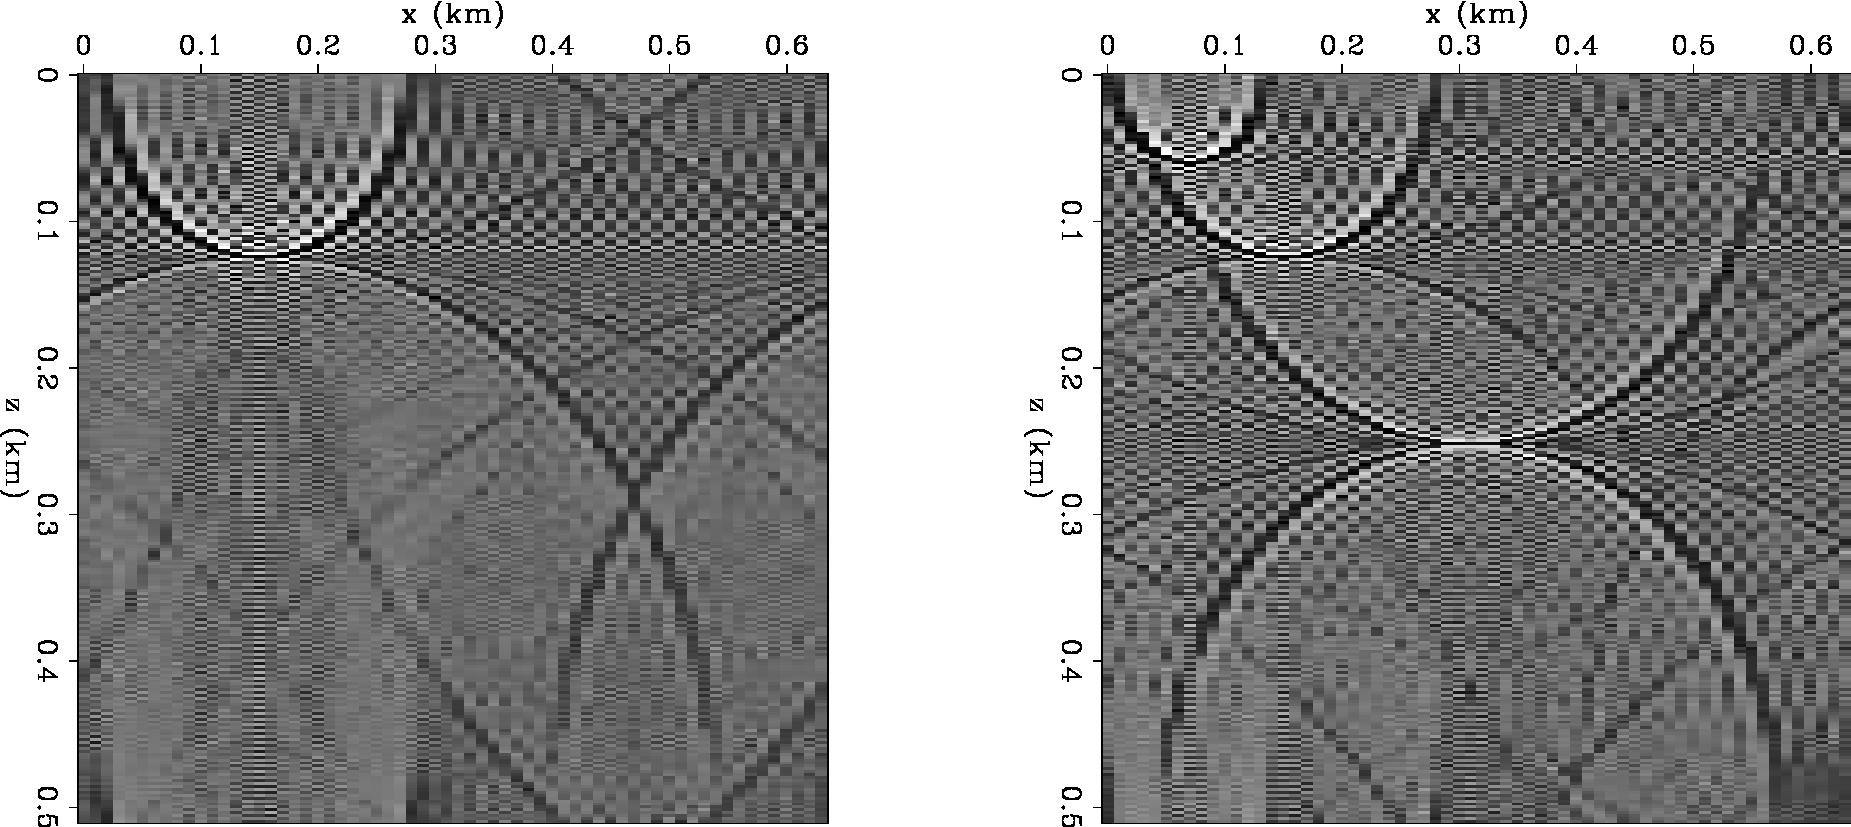
\includegraphics[width=0.95\textwidth]{omk/stolt}
\caption[stolt]{Stolt方法对脉冲数据的响应。可看到许多半圆弧与计算假象在一起}
\label{fig:omk/stolt}
\end{figure}
看来在时间轴上需要充填极其大量的零值,为保持合理的内存要求,可按习题(4)所
述算法重新加以组织。当然,$x$方向有周期性,所以沿$x$轴也需要充填零值。

\subsection{统射扫描法可改进为Kirchhoff法}
Schneider ( 1978 )证明惠更斯二次震源子波的解析表达式为\footnote{$step(t-r/v)$
为阶跃函数。——译者}
\begin{equation}
FT^{-1}(e^{ik_zz})=\frac{1}{\pi}\frac{\partial}{\partial z_0}\frac{step(t-r/v)}{\sqrt{t^2-r^2/v^2}}
\label{eq:ex1.3.10}
\end{equation}
式中,$r$为震源(爆炸反射面)与接收器之间的距离$\sqrt{x^2+(z-z_0)^2}$。函数
\ref{eq:ex1.3.10}中含有一项极点和阶跃函数的导数,由于趋于无限大,实际上是不可能
用图形来表示这个子波函数的。不过,根据其数学形式,你立刻回认识到扰动全部集中于所
期望的圆锥面上。在该锥面上,阶跃函数之导数给出一个正脉冲初至,平方根倒数之导数给出
一脉冲,其负极性之尾巴以$-3/2$次幂阻尼衰减。因为导数是对$z$求导而不是对$r$求导,
所以会出现余弦倾斜因子。

式\ref{eq:ex1.3.10}说明的是二维惠更斯子波而不是三维子波(在次要的枝节方面有一些
不同),虽然点源产生的波主要是球面波,可是弯曲地层的聚焦作用却主要是一种二维聚焦,
亦即,弯曲地层不像是球面而倒更像是柱面。

你也许会奇怪:为什么严格的逆变换\ref{eq:ex1.3.10}虽已知而不论谁却还是宁愿采用它
的近似。实践证明,以图形表示式\ref{eq:ex1.3.10}的困难表现在用它对数据资料进行褶
积时有困难,那也正是为什么普遍公认前述一些Kirchhoff偏移方法在平缓海底反射之上要出
现前兆干扰。第二章和第四章的内容大部分是用于讨论将式\ref{eq:ex1.3.10}推广至变速
情形下也能成立,以及将它推广成为数据网格上比较好的表现形式。

在傅氏变换域内,惠更斯二次震源函数很简单而且足平滑的,在矩形网格上计算该函数然后采用
1.7节所述程序进行逆变换,是一桩简易的事,图\ref{fig:omk/huygens}所示是在一个
$256\times 64$网格点上的计算结果(在实际处理时,将采用大约是$1024\times 256$
的网格,但此处所采用之稀疏网格可提供一种具有适当细节的图形),因为以图形表示一个类似
于脉冲偶极子的函数有困难,在图\ref{fig:omk/huygens}的下部又显示了其时间积分的第
二种图形。
\begin{figure}[H]
\centering
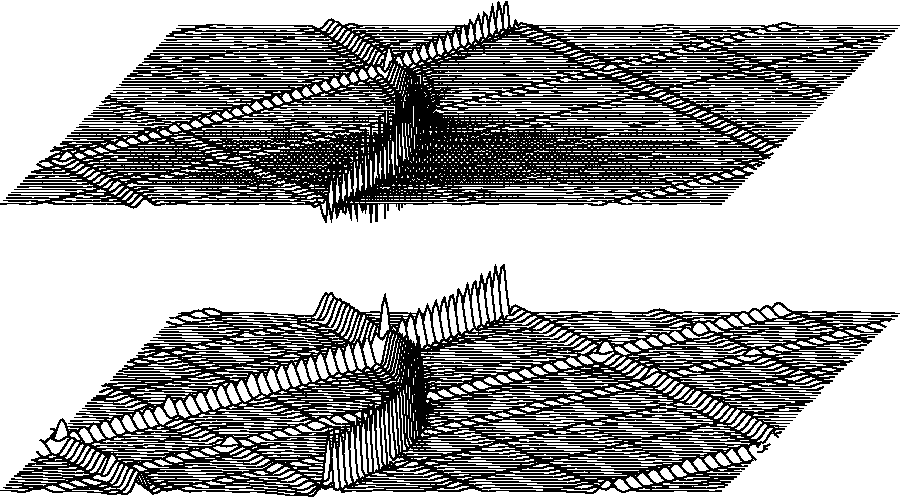
\includegraphics[width=0.95\textwidth]{omk/huygens}
\caption[huygens]{惠更斯子波(上图)及其平滑时间积分(下图)}
\label{fig:omk/huygens}
\end{figure}
\subsection{偏移方法对速度误差的灵敏度}
图\ref{fig:omk/sensitive}表示偏移的脉冲响应随速度如何变化的情形。注意,偏移资料
通常是以时间剖面形式显示的,对于水平成层情形,任何速度误差都没什么影响\footnote{根
据能量耗散率常数$1/Q$的定义:\\ 
$\frac{\pi}{Q}=\frac{\alpha}{f}$\\
其中,$\alpha$为衰减系数,$f$为波的频率。因主周期$\Delta T$与频率之关系为$\Delta T = \frac{1}{f}$,
故得即比值$\frac{T}{\Delta T}=\frac{\alpha T}{\pi}Q$,即比值$\frac{T}{\Delta T}$
与$Q$值有关。——译者}。
\begin{figure}[H]
\centering
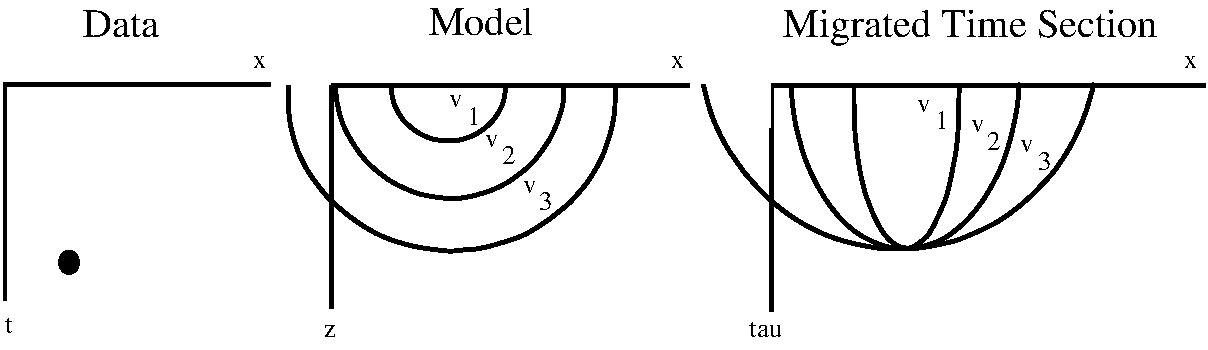
\includegraphics[width=0.95\textwidth]{omk/sensitive}
\caption[sensitive]{速度误差灵敏度随角度(可达$90^{\circ}$而增大。数据脉冲的偏移犹如是速度
之函数。三种可能的恒定速度选择均重叠显示在同一个平面上}
\label{fig:omk/sensitive}
\end{figure}
不同的人有不同的精确度准则,合理的准则应是:半圆弧上的能量之误差须小于半波长,对于沿
水平方向传播的能量来说,该项定位误差只与主周期$\Delta T$和旅行时间$T$有关\footnote{原文为“\ldots\ldots{}在间距是小于一个波长的情形下,\ldots\ldots”,显系有误。如杲确系小于一个波长,则需\\
$\Delta x=\frac{1}{2}Tsin\theta\Delta v<\lambda=v\Delta T$\\
从而\\
$\frac{\Delta v}{v}<\frac{2}{sin\theta}(\frac{\Delta T}{T})$\\
当$\theta=\pi/2$及$\Delta T/T=0.01$时,应有$\frac{\Delta v}{v}<2\frac{\Delta T}{T}=0.02$,
这个结果显然与$\theta=\pi/2$时“速度误差必须小于百分之一 ”的结论自相矛盾。由此可知,
所谓“小于一个波长”显然是“小于半个波长”之误。}。比值$\Delta T/T$超过$100$是难得见的,
看来这项数值$100$似乎是沉积岩的一种反射地震学基本观测参量(从理论上说,它也许与沉积岩的
“Q值”有关,或者,它可能与产生无序的层内多次反射有关系;在下列情形时出现高于100的大值:
(1)传播路程大部分均位于水层中时;(2)位于大于4秒左右的时间深度上时)。图\ref{fig:omk/senser}
是两种相近的偏移速度情形的比较,由图可知,两种曲线之间的间距随角度之增大而增大。在间距是小于半个
波长的。情形下,对于90°的角度,速度误差必须小于一百分之一;对于$45^{\circ}$倾角,偏移
速度误差可比它大$\sqrt{2}$倍\footnote{在偏移平面$(x,\tau)$内的等时线方程为\\
$\frac{4x^2}{v^2T^2}+\frac{\tau^2}{T^2}=1$\\
由此可得
$\tau=T\sqrt{1-\frac{4x^2}{v^2T^2}}=T\sqrt{1-sin^2\theta},x=\frac{1}{2}vTsin\theta (i)$
式中,$T$为双程传播时间,$\theta$为图\ref{fig:omk/senser}所示偏移方向与垂直方向之间的夹角。
根据定义(i),因速度$v$有误差$\Delta v$而形成之定时误差$\Delta \tau$与定位误差$\Delta x$
为\\
$\Delta \tau=T(\frac{4x^2\Delta v}{v^3T^2}/\sqrt{1-\frac{4x^2}{v^2T^2}})=T
sin\theta tan\theta(\frac{\Delta v}{v})$\\
$\Delta x = \frac{1}{2}Tsin\theta\Delta v$\\
或者\\
$\frac{\Delta\tau}{T}=sin\theta tan\theta(\frac{\Delta v}{v}) (ii)$\\
$\frac{\Delta x}{vT}=\frac{1}{2}sin\theta(\frac{\Delta v}{v}) (iii)$\\
由此可知:
\begin{enumerate}
\item 相对定时误差$\Delta \tau/T$与相对定位误差$\Delta x/vT$对相对速度误差$\Delta v/v$之灵敏度分别为$sin\theta tan\theta$与$(sin\theta)/2$,二者均随角$\theta$之增大而增大;
\item 对于固定的速度误差定时误差$\Delta v/v$随角度$\theta$之增大而增大;
\item 对于水平成层情形$\theta=0$,因$\Delta\tau=0$及$\Delta x=0$,从而既无定时误差亦无定位误差。
设$\lambda$为波长,$\Delta T$为主周期,即$\lambda=*v\Delta T$。若定位误差$\Delta x$小于半波长,即\\
$\frac{1}{2}Tsin\theta\Delta v<\frac{\lambda}{2}=\frac{1}{2}v\Delta T$,则\\
$\frac{\Delta v}{v}<\frac{1}{sin\theta}(\frac{\Delta T}{T} ) (iv)$\\
由式(iv)又可得结论:
\begin{enumerate}
\item 对于沿水平方向$\theta=\pi/2$传播的能量,应有\\
$\frac{\Delta v}{v}<\frac{1}{sin(\frac{\pi}{2})}(\frac{\Delta T}{T})=\frac{\Delta T}{T}$\\
亦即$\theta=\pi/2$时的速度误差$\Delta \theta=\pi/2$仅与主周期$\Delta T$和旅行时间$T$有关;
\item   $\Delta T/T$值一般为0.01,因此,在$\theta=\pi/2$的情形下,相对速度误差$\Delta v/v$必须小于0.01;
\item   由式(iv)可知,当$\theta=\pi/4$时,应有$\frac{\Delta v}{v}<\sqrt{2\frac{\Delta T}{T}}$,亦即$\theta=\pi/4$时的速度误差可比$\theta=\pi/2$时的速度误差大$\sqrt{2}$倍。——译者
\end{enumerate}
\end{enumerate}
}。
\begin{figure}[H]
\centering
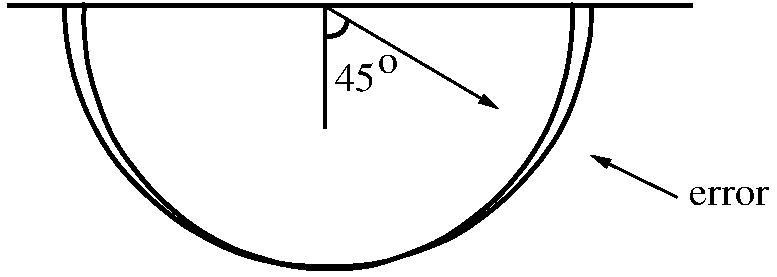
\includegraphics[width=0.6\textwidth]{omk/senser}
\caption[senser]{速度错误时的定位误差随角度而增大}
\label{fig:omk/senser}
\end{figure}

速度极少可精确已知到这神程度,所以我们可以怀疑广角偏移的价值。
\subsection{各种方法之比较与评价 }
本节所述偏移的三种方法,比较如下:
\newcolumntype{Y}{>{\centering\arraybackslash}X}
\begin{table}[!ht]
\centering
\ttfamily
\small
\begin{tabularx}{\textwidth}{Y|Y|Y|Y}
%\begin{tabular}{p{3cm}p{4cm}p{4cm}p{5cm}}
%\toprule
\hline 
 & 绕射扫描与等时线扫描法 & 相移法 & Stolt 法\\
%\midrule
\hline
运算速度 &慢 & 中等 & 极快\\ \hline
内存分配组织 & 不方便 & 良好 & 良好\\ \hline
垂向速度$v(z)$ & 采用射线追踪法& 易处理 & 采用拉伸方法近似处理\\ \hline
广角偏移有何问题? & 谨防数据假频与
					算子假频
 & 谨防数据假频 & 谨防数据假颏\\ \hline
是否需相位校正与
倾斜校正?
 & 在恒速情形下,可能
需作一些努力
 & 对任何$v(z)$均易于处理 &
在恒速情形下须作校正\\ \hline
有无$f-k$域假频干扰? & 无 & 在X轴上有干扰,减弱$t$
轴上干扰的方法见4.5节 &
在$x$轴上有干扰,减弱$(t,z)$
中的干扰的方法见4.5节\\ \hline
水平速度$v(x)$
 & 可使生产程序存在
严重的隐患
 & 可用迭代法与内插
方法近似处理 &
尚无已知的程序可处理\\ \hline
能否消除边界影响与不
规则采样间隔影响? & 极佳 & 差 & 差\\ \hline
%\bottomrule
\end{tabularx}
%\end{tabular}
\end{table}

展望以后几章的内容有可能对做为一类方法的各种广角偏移的质量作些注记,现在就作
一点评论将是有帮助的.这类方法最大的弱点就是它们难以处理横向速度变动问题;它
们的最大优点是处理广角的能力,但是却被数据采集与处理中其他环节的弱点所削弱。
这些弱点即:
\begin{enumerate}
\item   炮检距所张角度往往很大,而各种方法却均忽略了它的影响.CDP叠加剖面并非
  零炮检距剖面;
\item 甚至连垂直于测线方向的微小倾角都是忽略不计时,何必再去处理沿测线方向见
到的非常大的广角呢\footnote{意即垂直于测线方向的倾角对沿测线走向的视倾角有很
大影响,而前者在处理中常被忽略不计。——译者}
\item 数据总是采样密度不够,不足以代表陡倾斜资料而又无假频现象;
\item 速度资料的精度低,极难证明对广角进行处理的正确性;
\item 噪音干扰可能会压制掉所有回声反射,而这也就意味着存在有-种截止倾角了。
例如,试想像在两秒的时间深度上有含油储层,该处的数据记录则停止在四秒的时间
上,这意味着倾角在60°时就截止了\footnote{偏移时间剖面为$(x,\tau)$平面,未
偏移时间剖面为$(x,T)$平面,时间剖面上的时间深度为相应的偏移时间深度为$T$,二
者存在下列关系:$\tau=Tcos\theta$,其中,$\theta$为偏移角度,当$\tau=2$秒,
$T=4$秒时,应得$\theta=\pi/3$。——译者}。
\end{enumerate}
\subsection{习题}
\begin{enumerate}
\item 波动模拟程序流程简图均假设爆炸反射面为时间的脉冲函数,试修改程序流程简
图使波动模拟能包括一项震源波形$s(t)$
\item 偏移程序流程简图允许速度随深度而变化,然而当速度是恒定的深度函数时却可
相当快地提高程序的运算效率,试证明如何可作到这一点。
\item 试作出Stolt算法逆过程的程序流程——就是说,根据一已知模型作出合成记录。
\item Stolt算法可加以重新组织,使得沿$x$轴充零时所需要的内存得以减少。首先沿$x$轴
  进行傅氏变换,变换至$k_x$域,然后从数据所在$(t,k_x)$平面选择恒定$k_x$值的向量;可将每
  个向量移至某一长向量的空间内,然后进行充零和内插。试作出所述程序的流程图。
\item 已知地震资料是在四秒处截止,试问可观测到80°倾角的最深旅行时间深度是多少?
\end{enumerate}
